Em 1995, Robert McCool e seu grupo de pesquisa desenvolveram o servidor web Apache. O nome originou-se de uma tribo indígena de mesmo nome. O Apache é um software livre, ou seja, possui um código aberto, distribuído sob a licença GNU, ou seja, é gratuito e pode ser estudado e modificado através de seu código fonte por qualquer pessoa. Além disso, é o servidor da web mais popular desde abril de 1996 \cite{netcraft}.

Segundo \citeonline{apache:webmedia}, o servidor web Apache é projetado para trabalhar com uma ampla variedade de plataformas e ambientes. Isto é possível devido à sua implementação  modular. Introduzindo modelos de processos MPM (Multi-Processing-Modules), responsáveis por gerenciar as portas de comunicação, aceitar conexões e alocar processos ou \textit{threads} para atendimento das requisições.

Como \citeonline{apache:Marcelo} fala em seu artigo, o Apache é \textit{open source}, multi-plataforma mais utilizado em todo o mundo. As principais características do Apache são flexibilidade, altamente configurável, robustez, escalabilidade, pode ser configurado para diferentes funções e é composto de módulos separados onde cada um implementa uma característica diferente.

\citeonline{apache:magazine} comenta em uma edição da revista Infra Magazine que a excelência desta aplicação e a qualidade que um software \textit{open source} pode obter quando possui um desenvolvimento maduro e sério. O principal fator relacionado à performance é o número de instâncias do servidor. O Apache suporta um grande número de instâncias simultâneas, onde cada uma é relacionada a um cliente acessando o servidor, oferecendo também suporte a módulos que, quando instalados, adicionam funcionalidades ao servidor. Como exemplos, pode-se citar o \textit{mod\_php}, \textit{mod\_python}, \textit{mod\_ftp}, entre outros, o que permite que os usuários escrevam seus próprios módulos por meio da API do software.

O Apache é composto por módulos (\autoref{fig:modularizacaoApache}) para segurança, cache, reescrita de URL, autenticação de senhas e mais. O módulo denominado de \textit{mod\_ssl} por exemplo, adiciona a capacidade do servidor de atender solicitações usando o protocolo HTTPS. Este protocolo faz uso da camada SSL para a criptografia de todos os dados transferidos, proporcionando maior segurança entre o tráfego de dados entre cliente e servidor,  disponibilizado para Windows, Novell Netware, OS/2 e outros sistemas do padrão POSIX, como o Unix e o Linux, onde é amplamente utilizado \cite{apache:magazine}.

\begin{figure}[H]
    \centering
    \caption{Modularização Apache}
    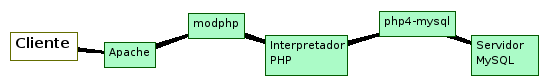
\includegraphics[width=0.9\textwidth]{./dados/figuras/fig12}
    \fonte{\citeonline{modapache}}
    \label{fig:modularizacaoApache}
\end{figure}

%%% Por exemplo, quando você acessa uma página em PHP em um site que roda sobre um servidor Apache, ele (Apache) lê o arquivo no disco e repassa a requisição para o modphp, o módulo encarregado de processar arquivos PHP. Ele, por sua vez, aciona o interpretador PHP, que processa a página e a entrega, já processada, ao Apache, que, finalmente, a entrega ao cliente. Caso seja necessário acessar um banco de dados (como no caso de um fórum), entra em ação outro módulo, como o php4-mysql, que permite que o interpretador PHP acesse o banco de dados:

%https://canaltech.com.br/internet/O-que-e-servidor-Apache/
%https://www.hostinger.com.br/tutoriais/o-que-e-apache
%https://www.weblink.com.br/blog/o-que-e-apache